%----------------------------------------------------------------
%
%  File    :  survey-design.tex
%
%  Author  :  Keith Andrews, IICM, TU Graz, Austria
% 
%  Created :  27 May 1993
% 
%  Changed :  03 Feb 2017
% 
%----------------------------------------------------------------


\chapter{Changes of the Design}

\label{chap:design}

The design of rSlidy has undergone numerous major changes throughout our project. A comparison between the old and the new version is given in this chapter.

\section{The Status Bar}
The initial version of rSlidy was equipped with a permanent status bar, as shown in Figure \ref{fig:statusbarOLD}.

It has been modified in terms of design and functionality. The final appearance of the status bar is shown in  Figure \ref{fig:statusbarNEW}. The following individual changes have been made.

\begin{figure}[tp]
	\centering
	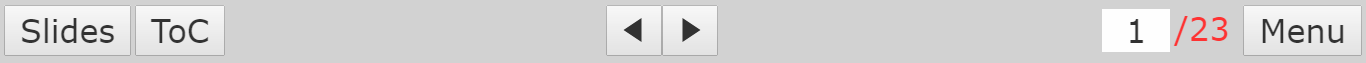
\includegraphics[width = \textwidth]{images/status_bar_old.png}
	
	\caption[Original Status Bar]{
		Design of rSlidy's original status bar.
		\imgcredit{Screenshot taken by the authors of this survey.}
	}
	\label{fig:statusbarOLD}
\end{figure}

\begin{figure}[tp]
	\centering
	\includegraphics[width = \textwidth]{images/status_bar_NEW.png}
	
	\caption[Modified Status Bar]{
		Design of rSlidy's modified status bar.
		\imgcredit{Screenshot taken by the authors of this survey.}
	}
	\label{fig:statusbarNEW}
\end{figure}


\subsection{Progress Bar}
A simple blue progress bar has been added on top of the status bar. Its purpose is to give some visual feedback about the current progress within a presentation. Its implementation is fairly simple.

A progress bar container was added at the desired position whose width property is changed on each slide change (see Listing \ref{list:progressbar}).


\begin{lstlisting}[
language=JavaScript,
label=list:progressbar,
caption={[Progress Bar Width Adaptation] Adapting width of the progress bar container for authentic visual feedback %
\imgcredit{The 
code example is based 
on the users' implementation.}
}
]
Rslidy.prototype.showSlide = function (slide_index) {
	// ...
	var progress_bar = document.getElementById("progress-bar");
	progress_bar.style.width =
				'calc(100%*' + (slide_index + 1) / this.num_slides + ')';
	// ...
}
\end{lstlisting}

\subsection{Rearrangement / Extension of the Navigation Elements}
We found it simply more intuitive to have the input field for jumping to a specific slide in the middle of the forward / backward buttons.

Apart from this, functionalities to jump to the first respectively the last slide have been added. These two starightforward implementations can be seen in Listing \ref{list:firstlastslide}.

\begin{minipage}{\linewidth}
\begin{lstlisting}[
language=JavaScript,
label=list:firstlastslide,
caption={[First / Last Slide Buttons Implementation] Implementation of the buttons for jumping to the first / last slide%
\imgcredit{The 
code example is based 
on the users' implementation.}
}
]
document.getElementById("status-bar-nav-button-first")
	.addEventListener('click', function ()
	{
		this.showSlide(0);
	}.bind(this));
document.getElementById("status-bar-nav-button-last")
	.addEventListener('click', function ()
	{
		this.showSlide(this.num_slides - 1);
	}.bind(this));
\end{lstlisting}
\end{minipage}



\subsection{Pin Functionality}
In opposition to the original rSlidy status bar, the new one features pinning / unpinning. The pinned status bar works the same as the old one. The unpinned status bar disappears when not hovering over it. When the mouse is not close to the bottom of the document, only the progress bar is visible in the unpinned mode. Two subtle triangles have been added to the unpinned status bar which are meant to function as little indicators for the actual bar. This implementation may not be the most elegant one, because it is relying on the title of the button to work properly. Some simple boolean variable which describes whether the bar is pinned or not may be a more robust solution. Still, this (see Listing \ref{list:pin_unpin}) is what we came up with and it works fine as long as the title tag of the pin button in the rslidy.js file is either "Pin the status bar" or "Unpin the status bar" (depending on whether the user wants the bar to be pinned or not by default).


\begin{minipage}{\linewidth}
\begin{lstlisting}[
language=JavaScript,
label=list:pin_unpin,
caption={[Pin / Unpin Implementation] Implementation of the buttons for pinning / unpinning the status bar %
\imgcredit{The 
code example is based 
on the users' implementation.}
}
]
Rslidy.prototype.pinToggleClicked = function (close_only) {
	var pin_button = document.getElementById("status-bar-pin-button");
	var status_bar = document.getElementById("status-bar-content");
	var indicator_left = document.getElementById("progress-bar-indicator-left");
	var indicator_right = document.getElementById("progress-bar-indicator-right");

	if (pin_button.title == "Pin the status bar")
	{
		pin_button.title = "Unpin the status bar";
		status_bar.style = "transform: translateY(0);";
		pin_button.style.WebkitTransition = 'opacity 0.3s';
		pin_button.style.MozTransition = 'opacity 0.3s';
		pin_button.style.opacity = 0.5;
		indicator_left.style.visibility = "hidden";
		indicator_right.style.visibility = "hidden";
	}
	else
	{			
		pin_button.title = "Pin the status bar";
		status_bar.removeAttribute('style');
		pin_button.style.opacity = 1;
		indicator_left.style.visibility = "visible";
		indicator_right.style.visibility = "visible";
	}
};
\end{lstlisting}
\end{minipage}

\subsection{Buttons animations}
Similar to an animated hamburger icon, which changes its shape on click, the buttons within the status bar of rSlidy are animated now as well. Listing \ref{list:buttonflip} shows how the animated flip was created. These style changes and the button's text changed to an "X" lead to a simple and intuitive animation of a button which turns around to change its functionality. 

\begin{minipage}{\linewidth}
	\begin{lstlisting}[
	language=CSS,
	label=list:buttonflip,
	caption={[Flip Button Animation] Implementation of the animation of the buttons in the status bar %
	\imgcredit{The 
	code example is based 
	on the users' implementation.}
	}
	]
#button-overview, #button-toc, #button-menu{ 
	animation-duration: 0.3s; 
	animation-timing-function: ease-in-out;
	animation-fill-mode: forwards;
	animation-name: flip2Face;
}

#button-overview.clicked, #button-toc.clicked, #button-menu.clicked{
	animation-name: flip2Back; 
	transform: rotateY(180);
}
	\end{lstlisting}
\end{minipage}






\section{The Menu}
The menu has been modernized and harmonized as seen in a direct comparison of Figure \ref{fig:menuOLD} and Figure \ref{fig:menuNEW}.

\begin{figure}[tp]
	\centering
	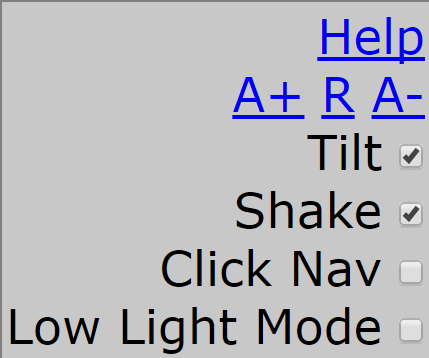
\includegraphics[width = .4\textwidth]{images/menu_old.png}
	
	\caption[Original Menu]{
		Design of rSlidy's original menu.
		\imgcredit{Screenshot taken by the authors of this survey.}
	}
	\label{fig:menuOLD}
\end{figure}

\begin{figure}[tp]
	\centering
	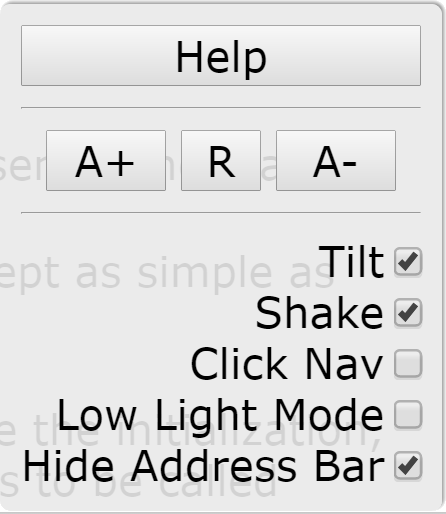
\includegraphics[width = .4\textwidth]{images/menu_new.png}
	
	\caption[Modified Menu]{
		Design of rSlidy's modified menu.
		\imgcredit{Screenshot taken by the authors of this survey.}
	}
	\label{fig:menuNEW}
\end{figure}

Implementation-wise these changes were mostly straightforward:
\begin{itemize}
	\item Partial transparency has been added to the menu. The actual document thus slightly shines through the menu.
	\item The corners have been corners in order to get a smoother look in general.
	\item Shadow effects have been added to the edges of the menu in order to get a very basic 3D-effect.
	\item Harmonization has taken place. All links were exchanged with buttons. This means more consistency in the design altogether. 
	\item One more checkbox has been added. It allows the user to switch between a version which, as usual, shows the address of a link on hover and a version which suppresses that standard function by removing the "href" property from all initial links.
\end{itemize}


\section{The Help Information}
This information, which can be opened from the menu, used to be a usual alert box. Due to the instructor's wish to have no third party libraries included, there are two versions of our implementation for the new help popup.

The initially intended version is based on a library called "sweetalert" (\url{https://limonte.github.io/sweetalert2/}). It allows animated popup messages with focusing on the actual text. The advantage of this way of implementation is the the polished design while having to rely on a third party library. 

The revised version simply opens a new tab to display the help message. This does not look as sophisticated as the other version, but still works fine and is an independent way of solving the popup problem.
